\section{Another CQs fail Example}
\label{app:toy-cq-fail}
In this section, we consider the following 2D minimization problem:
\begin{align}
    \label{eq:case:problem}
    \min_{x_1,x_2} & \displaystyle \,\,\,x_1 \notag\\
    \subject &\,\, x^3_1-x_2 \geq 0,\\
    & \,\, x^3_1+x_2 \geq 0.\notag
\end{align}
The objective level set and the feasible region are visualized in \prettyref{fig:prob_illustration}. From the figure, we shall easily observe that the optimal solution lies at $x^*=(0,0)$. Let the objective and the constraints in (\ref{eq:case:problem}) be $f(x)$, $c_1(x)$ and $c_2(x)$ respectively, we have:

\begin{equation}
\nabla f\left(x\right)=\left[\begin{array}{l}
1 \\
0
\end{array}\right], \quad \nabla c_1\left(x\right)=\left[\begin{array}{c}
3x_1^2\\
-1
\end{array}\right], \quad \nabla c_2\left(x\right)=\left[\begin{array}{c}
3x_1^2 \\
1
\end{array}\right].
\end{equation}
At the optimal point $x^*$, the gradients of the two constraints are linearly dependent ($\nabla c_1(x^*)=[0,-1]^{\top}$ and $\nabla c_2(x^*)=[0,1]^{\top}$), causing the Linear Independence Constraint Qualification (LICQ) to fail. LICQ is typically required for the KKT system to provide necessary first-order optimality conditions~\cite{nocedal1999springer-numerical-optimization}. While alternative constraint qualifications exist that can yield analogous optimality conditions, a direct examination of the Lagrangian gradient $\nabla_x \mathcal{L}$ at the optimal point $x^*$ reveals the failure of the KKT conditions. Specifically, there exist no Lagrange multipliers $\lambda_1$ and $\lambda_2$ that satisfy:
\begin{equation}
    \nabla f(x^*) - \lambda_1 \nabla c_1(x^*) -\lambda_2 \nabla c_2(x^*) = \left[\begin{array}{c}
         1 \\
         \lambda_1 -\lambda_2 
    \end{array}\right] = \mathbf{0}.
\end{equation}
In this section, we conduct a comprehensive analysis of our proposed algorithm's performance on this typical problem, encompassing both theoretical investigation and numerical experiments.

\begin{figure}[htbp]
    \centering
    \includegraphics[width=0.2\textwidth, trim={5cm 9cm 5cm 9cm}, clip]{figures/toy_appendix.pdf}
    \caption{Visualization of the objective level sets (red lines) and the feasible region (shaded area).}
    \label{fig:prob_illustration}
\end{figure}
\paragraph{Convergency Analysis} Starting from an initial point $\boldsymbol{x}_0$, we implement Algorithm \ref{alg:sl1qp:modified} on the problem (\ref{eq:case:problem}) recursively to obtain a sequence of $\boldsymbol{x}$. Suppose we are now at $\boldsymbol{x}_k$, a trial step $\hat{\boldsymbol{p}}_k = [\hat{p}_{k,1},\hat{p}_{k,2}]$ at each iteration $k$ by solving:
\begin{align}\label{eq:case:subproblem_k}
\min_{\hat{\boldsymbol{p}}} \, & \quad x_1 + \hat{p}_1 + \mu[x_1^3-x_2+3x_1^2\hat{p}_1-\hat{p}_2]^- + \mu[x_1^3+x_2+3x_1^2\hat{p}_1+\hat{p}_2]^-\\
\subject & \quad \norm{\hat{\boldsymbol{p}}_k}_\infty \leq \Delta_k.\notag
\end{align}
For simplicity, we abbreviate the explicit dependence of certain variables on the iteration number $k$. Given that~\eqref{eq:sl1qp:sl1qp-subproblem} is merely a smooth reformulation of~\eqref{eq:case:subproblem_k} with an identical minimizer, we focus our analysis on the non-smooth version, which offers greater analytical tractability. The optimal trial step, which minimizes the objective function while adhering to the trust-region constraint, is contingent upon three key factors: the chosen penalty parameter $\mu$, the current position $(x_1, x_2)$, and the trust-region radius determined in the outer loop.




Denote the two penalty terms in~\eqref{eq:case:subproblem_k} as $m_{\mu}$, we rearrange it as:
\begin{equation}
    m_{\mu} = \mu[x_1^2(x_1+3\hat{p}_1)-(x_2+\hat{p}_2)]^- + \mu[x_1^2(x_1+3\hat{p}_1)+(x_2+\hat{p}_2)]^-.
\end{equation}
Given that the terms beyond $m_{\mu}$ are independent of $\hat{p}_2$, we first focus our analysis on determining the optimal value of $\hat{p}_2$ that minimizes $m_{\mu}$. From the symmetric characteristic of the two terms, we can infer that: 
\begin{align}
x_1 + 3p_1 \leq 0 &\Rightarrow \textbf{Take}\,\begin{array}{c}
     |x_2+\hat{p}_2| \leq -x_1^2(x_1 + 3\hat{p}_1)  \\
     \&\&\,|\hat{p}_2\leq\Delta_k|
\end{array} \Rightarrow \min m_{\mu}=2\mu(-x_1^2(x_1+3\hat{p}_1)), \label{eq:case:mu_1}\\
x_1 + 3p_1 > 0 &\Rightarrow \textbf{Take}\,\begin{array}{c}
     |x_2+\hat{p}_2| \leq x_1^2(x_1 + 3\hat{p}_1)  \label{eq:case:mu_2}\\
     \&\&\,|\hat{p}_2\leq\Delta_k|
\end{array} \Rightarrow \min m_{\mu}=0.
\end{align}

Note that if the set inside ``\textbf{Take}'' is $\emptyset$, then $p_2 = -\mathrm{sign}(x_2)\Delta_k$. This implies that the absolute value of $x_2$ is monotonically decreasing. Consequently, after a finite number of iteration, the set will become non-empty. 

Combining the cases in~\eqref{eq:case:mu_1} and~\eqref{eq:case:mu_2}, we rewrite the objective in~\eqref{eq:case:subproblem_k} by taking appropriate value on $\hat{p}_2$:
\begin{equation}
\label{eq:case:subproblem_k_min}
\min_{\hat{p}_1} \,  \quad x_1 + \hat{p}_1 - \min\{0,2\mu(x_1^2(x_1+3\hat{p}_1))\},
\end{equation}
where we can absorb all terms in the $\min$ operator and disregard the constant $x_1$ to further simplify it to a \textit{min-max} form:
\begin{equation}
\label{eq:case:subproblem_k_simplify1}
\min_{\hat{p}_1} \max\{\hat{p}_1,\hat{p}_1-2\mu(x_1^2(x_1+3\hat{p}_1))\},\,|\hat{p}_1|\leq \Delta_k.
\end{equation}
\begin{center}
$\downarrow$
\end{center}
\begin{equation}
\label{eq:case:subproblem_k_simplify2}
\min_{\hat{p}_1} \max\{\hat{p}_1,(1-6\mu x_1^2)\hat{p}_1-2\mu x_1^3\},\,|\hat{p}_1|\leq \Delta_k.
\end{equation}
\begin{figure}[ht]
  \centering
  \begin{subfigure}[b]{0.30\textwidth}
  \centering
%%%    \begin{adjustbox}{width=\linewidth} % rescale box
    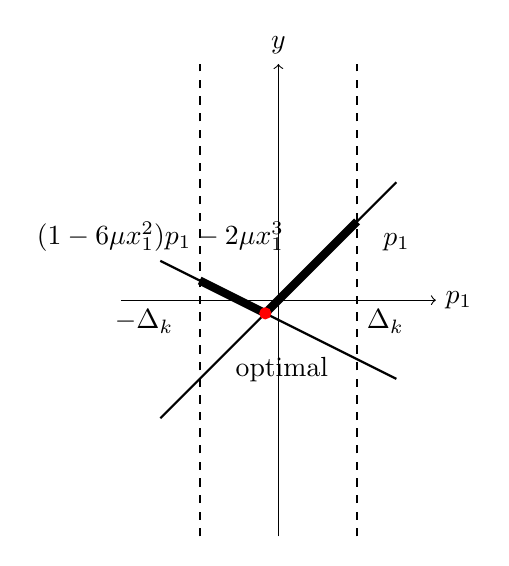
\begin{tikzpicture}
% Axes
    \draw[->] (-2,0) -- (2,0) node[right] {$p_1$}; % x-axis
    \draw[->] (0,-3) -- (0,3) node[above] {$y$}; % y-axis

    % Adjustable x1 value
    \def\xone{0.5} % Set x1 value (you can adjust this)

    % Vertical line for x = x1
    \draw[thick, dashed] (1,-3) -- (1,3); % x1 vertical line
    \node[below right] at (1,0) {$\Delta_k$};

    % Vertical line for x = x1
    \draw[thick, dashed] (-1,-3) -- (-1,3); % x1 vertical line
    \node[below right] at (-2.2,0) {$-\Delta_k$};

    % Line 1
    \draw[thick, domain=-1.5:1.5, samples=100] 
        plot (\x, {(1 - 6*(\xone)^2)*\x - 2*(\xone)^3}); % 
    \draw[line width=3pt, domain=-1:-\xone/3, samples=100] 
        plot (\x, {(1 - 6*(\xone)^2)*\x - 2*(\xone)^3});
    \node[above] at (-1.5,0.5) {$(1 - 6\mu x_1^2)p_1 - 2\mu x_1^3$};

    % Line 2
    \draw[thick, domain=-1.5:1.5, samples=100] 
        plot (\x, \x); 
    \draw[line width=3pt, domain=-\xone/3:1, samples=100] 
        plot (\x, \x);
    \node[above] at (1.5,0.5) {$p_1$};

     % Red point at (1, 1)
    \filldraw[red] (-\xone/3,-\xone/3) circle (2pt); % Draws a red filled circle at (1, 1)

    % Label for the red point
    \node[above right] at (-\xone/3-0.5,-\xone/3-1) {optimal };

    \end{tikzpicture}
%%%  \end{adjustbox}       %
\end{subfigure}%
   \hspace{0.02\textwidth}
  \begin{subfigure}[b]{0.30\textwidth}
  \centering
  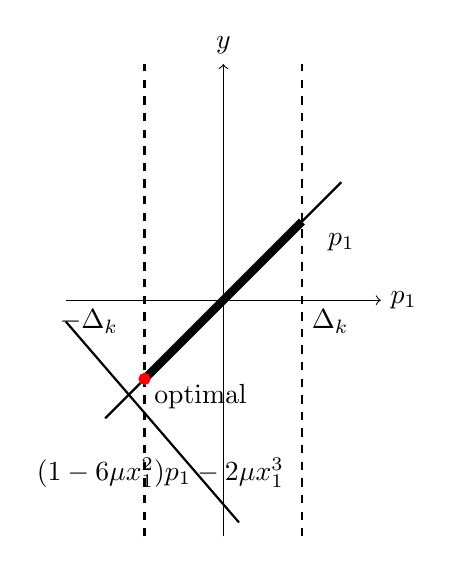
\begin{tikzpicture}
% Axes
    \draw[->] (-2,0) -- (2,0) node[right] {$p_1$}; % x-axis
    \draw[->] (0,-3) -- (0,3) node[above] {$y$}; % y-axis

    % Adjustable x1 value
    \def\xone{0.6} % Set x1 value (you can adjust this)

    % Vertical line for x = x1
    \draw[thick, dashed] (1,-3) -- (1,3); % x1 vertical line
    \node[below right] at (1,0) {$\Delta_k$};

    % Vertical line for x = x1
    \draw[thick, dashed] (-1,-3) -- (-1,3); % x1 vertical line
    \node[below right] at (-2.2,0) {$-\Delta_k$};

    % Line 1
    \draw[thick, domain=-2:0.2, samples=100] 
        plot (\x, {(1 - 6*(\xone)^2)*\x - 12*(\xone)^3}); % 
    \node[above] at (-0.8,-2.5) {$(1 - 6\mu x_1^2)p_1 - 2\mu x_1^3$};

    % Line 2
    \draw[thick, domain=-1.5:1.5, samples=100] 
        plot (\x, \x); 
    \draw[line width=3pt, domain=-1:1, samples=100] 
        plot (\x, \x);
    \node[above] at (1.5,0.5) {$p_1$};

     % Red point at (1, 1)
    \filldraw[red] (-1,-1) circle (2pt); % Draws a red filled circle at (1, 1)

    % Label for the red point
    \node[above right] at (-1,-1.5) {optimal };

    \end{tikzpicture}
%%%  \end{adjustbox}       %
\end{subfigure}%
\hspace{-0.01\textwidth}
\begin{subfigure}[b]{0.30\textwidth}
\centering
  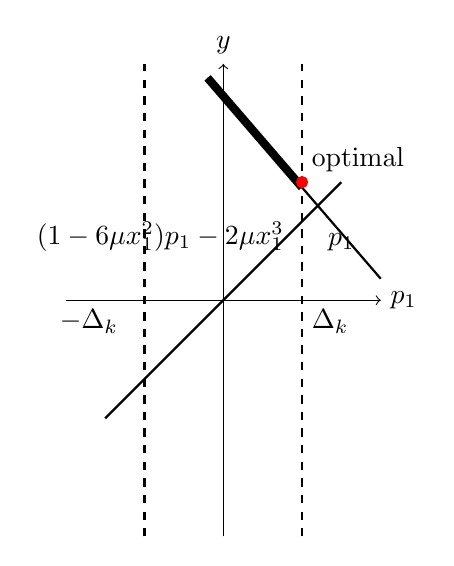
\begin{tikzpicture}
% Axes
    \draw[->] (-2,0) -- (2,0) node[right] {$p_1$}; % x-axis
    \draw[->] (0,-3) -- (0,3) node[above] {$y$}; % y-axis

    % Adjustable x1 value
    \def\xone{-0.6} % Set x1 value (you can adjust this)

    % Vertical line for x = x1
    \draw[thick, dashed] (1,-3) -- (1,3); % x1 vertical line
    \node[below right] at (1,0) {$\Delta_k$};

    % Vertical line for x = x1
    \draw[thick, dashed] (-1,-3) -- (-1,3); % x1 vertical line
    \node[below right] at (-2.2,0) {$-\Delta_k$};

    % Line 1
    \draw[thick, domain=-0.2:2, samples=100] 
        plot (\x, {(1 - 6*(\xone)^2)*\x - 12*(\xone)^3}); % 
      \draw[line width=3pt, domain=-0.2:1, samples=100] 
        plot (\x, {(1 - 6*(\xone)^2)*\x - 12*(\xone)^3});  
    \node[above] at (-0.8,0.5) {$(1 - 6\mu x_1^2)p_1 - 2\mu x_1^3$};

    % Line 2
    \draw[thick, domain=-1.5:1.5, samples=100] 
        plot (\x, \x); 

    \node[above] at (1.5,0.5) {$p_1$};

     % Red point at (1, 1)
    \filldraw[red] (1,1.5) circle (2pt); % Draws a red filled circle at (1, 1)

    % Label for the red point
    \node[above right] at (1,1.5) {optimal };

    \end{tikzpicture}
%%%  \end{adjustbox}       %
\end{subfigure}%
\caption{Visualization of cases where $1-6\mu x_1^2 \leq 0$. The graph illustrates three distinct scenarios, each corresponding to different values of $x_1$, showcasing the various intersections of the two linear functions. The bold segments represent the composite \textit{max} function, while the \textit{min} points are denoted by red dots. The intersection is $\hat{p}_1 = -x_1/3$.}
\label{fig:case-visualization01}
\end{figure}

\begin{figure}[H]
  \centering
  \begin{subfigure}[b]{0.30\textwidth}
  \centering
%%%    \begin{adjustbox}{width=\linewidth} % rescale box
    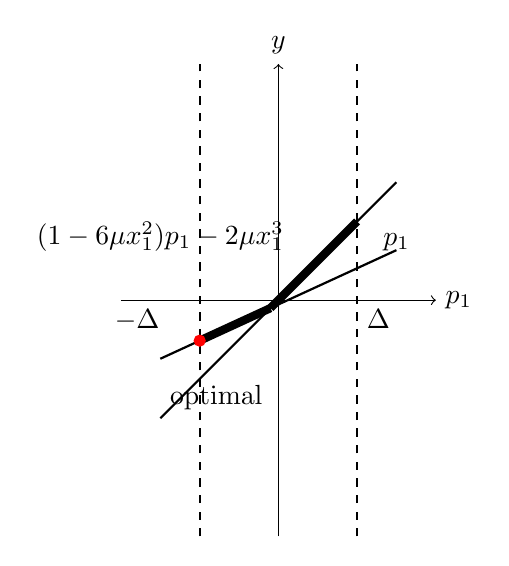
\begin{tikzpicture}
% Axes
    \draw[->] (-2,0) -- (2,0) node[right] {$p_1$}; % x-axis
    \draw[->] (0,-3) -- (0,3) node[above] {$y$}; % y-axis

    % Adjustable x1 value
    \def\xone{0.3} % Set x1 value (you can adjust this)

    % Vertical line for x = x1
    \draw[thick, dashed] (1,-3) -- (1,3); % x1 vertical line
    \node[below right] at (1,0) {$\Delta$};

    % Vertical line for x = x1
    \draw[thick, dashed] (-1,-3) -- (-1,3); % x1 vertical line
    \node[below right] at (-2.2,0) {$-\Delta$};

    % Line 1
    \draw[thick, domain=-1.5:1.5, samples=100] 
        plot (\x, {(1 - 6*(\xone)^2)*\x - 2*(\xone)^3}); % 
    \draw[line width=3pt, domain=-1:-\xone/3, samples=100] 
        plot (\x, {(1 - 6*(\xone)^2)*\x - 2*(\xone)^3});
    \node[above] at (-1.5,0.5) {$(1 - 6\mu x_1^2)p_1 - 2\mu x_1^3$};

    % Line 2
    \draw[thick, domain=-1.5:1.5, samples=100] 
        plot (\x, \x); 
    \draw[line width=3pt, domain=-\xone/3:1, samples=100] 
        plot (\x, \x);
    \node[above] at (1.5,0.5) {$p_1$};

     % Red point at (1, 1)
    \filldraw[red] (-1,-1 + 6*\xone^2 - 2*\xone^3) circle (2pt); % Draws a red filled circle at (1, 1)

    % Label for the red point
    \node[above right] at (-1.5,-1 + 6*\xone^2 - 2*\xone^3-1) {optimal };

    \end{tikzpicture}
%%%  \end{adjustbox}       %
\end{subfigure}%
   \hspace{0.02\textwidth}
  \begin{subfigure}[b]{0.30\textwidth}
  \centering
  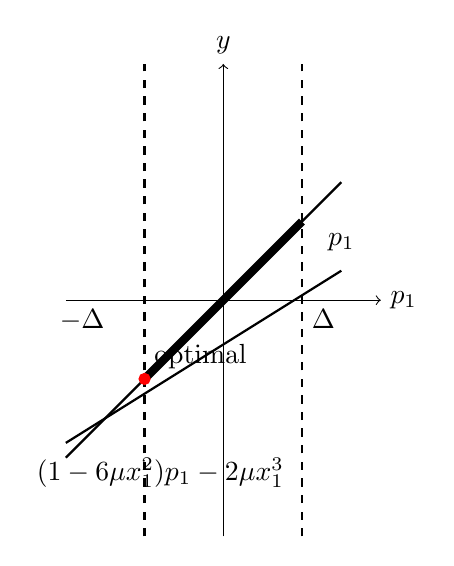
\begin{tikzpicture}
% Axes
    \draw[->] (-2,0) -- (2,0) node[right] {$p_1$}; % x-axis
    \draw[->] (0,-3) -- (0,3) node[above] {$y$}; % y-axis

    % Adjustable x1 value
    \def\xone{0.25} % Set x1 value (you can adjust this)

    % Vertical line for x = x1
    \draw[thick, dashed] (1,-3) -- (1,3); % x1 vertical line
    \node[below right] at (1,0) {$\Delta$};

    % Vertical line for x = x1
    \draw[thick, dashed] (-1,-3) -- (-1,3); % x1 vertical line
    \node[below right] at (-2.2,0) {$-\Delta$};

    % Line 1
    \draw[thick, domain=-2:1.5, samples=100] 
        plot (\x, {(1 - 6*(\xone)^2)*\x - 36*(\xone)^3}); % 
    \node[above] at (-0.8,-2.5) {$(1 - 6\mu x_1^2)p_1 - 2\mu x_1^3$};

    % Line 2
    \draw[thick, domain=-2:1.5, samples=100] 
        plot (\x, \x); 
    \draw[line width=3pt, domain=-1:1, samples=100] 
        plot (\x, \x);
    \node[above] at (1.5,0.5) {$p_1$};

     % Red point at (1, 1)
    \filldraw[red] (-1,-1) circle (2pt); % Draws a red filled circle at (1, 1)

    % Label for the red point
    \node[above right] at (-1,-1) {optimal };

    \end{tikzpicture}
%%%  \end{adjustbox}       %
\end{subfigure}%
\hspace{-0.01\textwidth}
\begin{subfigure}[b]{0.30\textwidth}
\centering
  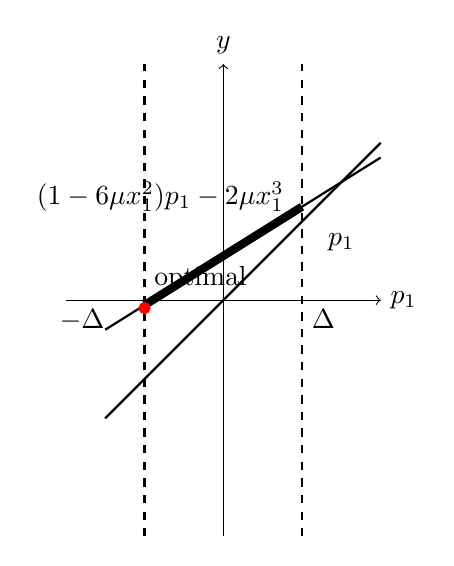
\begin{tikzpicture}
% Axes
    \draw[->] (-2,0) -- (2,0) node[right] {$p_1$}; % x-axis
    \draw[->] (0,-3) -- (0,3) node[above] {$y$}; % y-axis

    % Adjustable x1 value
    \def\xone{-0.25} % Set x1 value (you can adjust this)

    % Vertical line for x = x1
    \draw[thick, dashed] (1,-3) -- (1,3); % x1 vertical line
    \node[below right] at (1,0) {$\Delta$};

    % Vertical line for x = x1
    \draw[thick, dashed] (-1,-3) -- (-1,3); % x1 vertical line
    \node[below right] at (-2.2,0) {$-\Delta$};

    % Line 1
    \draw[thick, domain=-1.5:2, samples=100] 
        plot (\x, {(1 - 6*(\xone)^2)*\x - 36*(\xone)^3}); % 
      \draw[line width=3pt, domain=-1:1, samples=100] 
        plot (\x, {(1 - 6*(\xone)^2)*\x - 36*(\xone)^3});  
    \node[above] at (-0.8,1) {$(1 - 6\mu x_1^2)p_1 - 2\mu x_1^3$};

    % Line 2
    \draw[thick, domain=-1.5:2, samples=100] 
        plot (\x, \x); 

    \node[above] at (1.5,0.5) {$p_1$};

     % Red point at (1, 1)
    \filldraw[red] (-1,-0.1) circle (2pt); % Draws a red filled circle at (1, 1)

    % Label for the red point
    \node[above right] at (-1,0) {optimal };

    \end{tikzpicture}
%%%  \end{adjustbox}       %
\end{subfigure}%
\caption{Visualization of cases where $1-6\mu x_1^2 > 0$. In all three scenarios depicted, the optimal solution converges to the same \textit{min-max} point at $\hat{p}_1=-\Delta$, regardless of the specific intersection patterns of the linear functions.}
\label{fig:case-visualization02}
\end{figure}
We then analyze different cases distinguished by the sign of $1-6\mu x_1^2$. For clarity, these scenarios are illustrated in~\prettyref{fig:case-visualization01}, which provides an intuitive understanding of the process. The figure demonstrates how we first identify the \textit{max} segment of these two lines and then extract the \textit{min} point of the resulting composite line, thereby solving the constrained \textit{min-max} problem. Thus, we conclude that:
\begin{align}
|x_1| > 1/\sqrt{6\mu} &\Rightarrow \hat{p}_1  = \mathrm{clip}(\frac{-x_1}{3},\Delta_k) \\
-1/\sqrt{6\mu}\leq x_1 \leq 1/\sqrt{6\mu} &\Rightarrow \hat{p}_1  = -\Delta_k,
\end{align}
which indicates that $\hat{p}_1$ will always take a step towards $x_1=-1/\sqrt{6\mu}$, either with length $|x_1/3|$ or the trust region radius $|\Delta_k|$. The \textbf{clip} function is defined by $\mathrm{clip}(a,b) = \max\{\min\{a,b\},-b\}$. Consequently, $x_2$ would converge to zero by taking the value consistent in Equation~\eqref{eq:case:mu_1} and~\eqref{eq:case:mu_2}. We thus conclude that the proposed algorithm exhibits dynamic convergence towards a final stable point, $(-1/\sqrt{6\mu},0)$.

The radius of the trust region is dynamically adjusted based on the magnitude of decrease in the merit function induced by the trial step. Through a similar deduction on the merit function, with an appropriately chosen $x_2$, we obtain:
\begin{equation}
    \phi_1 = x_1 + \mu[x_1^3-x_2]^-+\mu[x_1^3+x_2]^- = 
    \begin{cases}
        x_1 - 2\mu x_1^3,  & \text{for } x_1 < 0 \\
        x_1, & \text{for } x_1 \geq 0
    \end{cases}
\end{equation}
The stationary point of $\phi_1$ is obtained at $x_1 = -1/\sqrt{6\mu}$ and $|x_2|\leq|x_1^3|$. In practice, we employ a large value for $\mu$, resulting in $x_2$ being a negligibly small quantity, approaching zero due to the cubic relationship. This stationary point aligns with the stable point of our algorithm.